\documentclass[11pt,a4paper]{article}
\usepackage[T1]{fontenc}
\usepackage{lmodern}
\usepackage{microtype}
\usepackage[margin=2.4cm]{geometry}
\usepackage{amsmath,amssymb,mathtools}
\usepackage{graphicx}
\usepackage{booktabs}
\usepackage{caption}
\usepackage{algorithm}
\usepackage{algpseudocode}
\usepackage{hyperref}
\usepackage{xcolor}
\usepackage{enumitem}
\usepackage{titlesec}
\usepackage{fancyhdr}

\newcommand{\NOne}{5}
\newcommand{\YBar}{1.80}
\newcommand{\PostMeanOne}{1.00000}
\newcommand{\PostSDOne}{0.33333}
\newcommand{\MHMean}{0.99361}
\newcommand{\MHSD}{0.32997}
\newcommand{\AcceptRate}{0.623}
\newcommand{\TotalStates}{10000}
\newcommand{\BurnIn}{1000}
\newcommand{\RetainedStates}{9000}
\newcommand{\Sxx}{17.50}
\newcommand{\Sxy}{9.00}
\newcommand{\PostMeanTwo}{0.50963}
\newcommand{\PostSDTwo}{0.09518}
\newcommand{\PriorCILow}{-1.95996}
\newcommand{\PriorCIHigh}{1.95996}
\newcommand{\PostCILow}{0.32307}
\newcommand{\PostCIHigh}{0.69618}


\hypersetup{colorlinks=true,linkcolor=black,urlcolor=blue,citecolor=black}
\captionsetup{font=small,labelfont=bf}
\setlength{\parindent}{0pt}
\setlength{\parskip}{0.65em}
\setlength{\headheight}{14pt}
\setlist{nosep}
\pagestyle{fancy}
\fancyhf{}
\fancyhead[L]{Bayesian Inference and Metropolis--Hastings}
\fancyhead[R]{\thepage}
\renewcommand{\headrulewidth}{0.4pt}

\title{Bayesian Inference with Metropolis--Hastings\\[0.4em]\large Theory and Two Analytically Checkable Examples}
\author{}
\date{}

\begin{document}
\maketitle
\tableofcontents
\newpage

\part{Theory}

\section{Bayesian inference}
Let \(\theta\) denote a parameter and let \(y\) denote observed data. A Bayesian model specifies a prior density \(p(\theta)\) and a sampling distribution \(p(y\mid\theta)\). Bayes' rule gives
\begin{equation}
 p(\theta\mid y)=\frac{p(y\mid\theta)p(\theta)}{p(y)},
 \qquad
 p(y)=\int p(y\mid\theta)p(\theta)\,d\theta.
 \label{eq:bayes}
\end{equation}
The posterior density \(p(\theta\mid y)\) describes uncertainty about \(\theta\) after observing \(y\). The evidence \(p(y)\) is a normalizing constant with respect to \(\theta\).

For conditionally independent observations \(y=(y_1,\ldots,y_n)\),
\begin{equation}
 p(y\mid\theta)=\prod_{i=1}^{n}p(y_i\mid\theta),
 \qquad
 \log p(y\mid\theta)=\sum_{i=1}^{n}\log p(y_i\mid\theta).
 \label{eq:iidlikelihood}
\end{equation}
The assumption is conditional independence given \(\theta\), not necessarily marginal independence.

A posterior expectation is a property of the posterior distribution. For a function \(g\),
\begin{equation}
 \mathbb{E}[g(\theta)\mid y]=\int g(\theta)p(\theta\mid y)\,d\theta.
 \label{eq:postexpectation}
\end{equation}
The distribution \(p(\theta\mid y)\) and the scalar summary \(\mathbb{E}[\theta\mid y]\) are distinct mathematical objects.

\section{Metropolis--Hastings sampling}
Metropolis--Hastings (MH) constructs a Markov chain whose stationary distribution is a target density \(\pi(\theta)\). In Bayesian inference, the target is usually the posterior. The method only requires an unnormalized density \(\widetilde\pi(\theta)\propto\pi(\theta)\), so the evidence in Equation~\eqref{eq:bayes} does not need to be evaluated.

A proposal density \(q(\theta'\mid\theta)\) generates a candidate \(\theta'\) from the current state \(\theta\).

\begin{algorithm}[ht]
\caption{Metropolis--Hastings with burn-in}
\label{alg:mh}
\begin{algorithmic}[1]
\Require Unnormalized target \(\widetilde\pi\); proposal density \(q\); initial state \(\theta^{(0)}\) with \(\widetilde\pi(\theta^{(0)})>0\); total number of states \(T\); burn-in limit \(B\), where \(0\le B<T\).
\For{\(t=0,1,\ldots,T-2\)}
    \State Generate \(\theta'\sim q(\cdot\mid\theta^{(t)})\).
    \State Compute
    \[
      R=\frac{\widetilde\pi(\theta')q(\theta^{(t)}\mid\theta')}
      {\widetilde\pi(\theta^{(t)})q(\theta'\mid\theta^{(t)})}.
    \]
    \State Set \(\alpha=\min\{1,R\}\).
    \State Generate \(U\sim\operatorname{Uniform}(0,1)\), independently of the proposal.
    \If{\(U\le\alpha\)}
        \State \(\theta^{(t+1)}\gets\theta'\). \Comment{accept}
    \Else
        \State \(\theta^{(t+1)}\gets\theta^{(t)}\). \Comment{reject and repeat the current state}
    \EndIf
\EndFor
\State Discard \(\theta^{(0)},\ldots,\theta^{(B-1)}\).
\State \Return \(\theta^{(B)},\ldots,\theta^{(T-1)}\).
\end{algorithmic}
\end{algorithm}

The uniform draw implements acceptance with probability \(\alpha\): for \(0\le\alpha\le1\), \(\Pr(U\le\alpha)=\alpha\). Rejected candidates are represented by repeated states and must remain in the chain.

The burn-in limit \(B\) specifies the initial states excluded from posterior estimation. These states can retain a strong dependence on the selected initial value before the chain reaches the region where the target density has substantial mass. Burn-in does not remove autocorrelation and does not by itself establish convergence; it only excludes a chosen initial transient.

\subsection{Detailed balance and stationarity}
For distinct states, the move density of the MH transition kernel is
\begin{equation}
 K(\theta,\theta')=q(\theta'\mid\theta)\alpha(\theta,\theta'),
\end{equation}
where
\begin{equation}
 \alpha(\theta,\theta')=
 \min\left\{1,
 \frac{\pi(\theta')q(\theta\mid\theta')}
 {\pi(\theta)q(\theta'\mid\theta)}\right\}.
\end{equation}
The acceptance probability is chosen so that
\begin{equation}
 \pi(\theta)K(\theta,\theta')=
 \pi(\theta')K(\theta',\theta).
 \label{eq:detailedbalance}
\end{equation}
Both sides of Equation~\eqref{eq:detailedbalance} equal
\begin{equation}
 \min\{\pi(\theta)q(\theta'\mid\theta),\,
 \pi(\theta')q(\theta\mid\theta')\}.
\end{equation}
This is the detailed-balance condition: under \(\pi\), probability flow from \(\theta\) to \(\theta'\) equals the reverse flow. Integrating over the starting state shows that \(\pi\) is stationary. Irreducibility and aperiodicity are additionally required for convergence to that stationary distribution from a general initial state.

For a symmetric proposal, \(q(\theta'\mid\theta)=q(\theta\mid\theta')\), and the proposal terms cancel. A Gaussian random-walk proposal has the form
\begin{equation}
 \theta'=\theta^{(t)}+\eta_t,
 \qquad \eta_t\sim\mathcal N(0,s_q^2),
\end{equation}
with acceptance ratio
\begin{equation}
 R=\frac{\widetilde\pi(\theta')}{\widetilde\pi(\theta^{(t)})}.
\end{equation}

\section{Bayesian inference with Metropolis--Hastings}
For Bayesian inference, set
\begin{equation}
 \widetilde\pi(\theta)=p(y\mid\theta)p(\theta).
 \label{eq:bayestarget}
\end{equation}
Because the evidence \(p(y)\) is common to all parameter values, it cancels from the Hastings ratio. After burn-in, posterior expectations may be estimated by sample averages:
\begin{equation}
 \mathbb{E}[g(\theta)\mid y]
 \approx \frac{1}{T-B}\sum_{t=B}^{T-1}g(\theta^{(t)}).
 \label{eq:mcmcaverage}
\end{equation}
The approximation is based on correlated Markov-chain states, not independent posterior samples. Consequently, Monte Carlo precision depends on the chain's autocorrelation as well as on the number of retained states.

\section{Forward models, additive errors, and residual likelihoods}
Suppose a deterministic model predicts
\begin{equation}
 y_i=f_i(\theta)+\varepsilon_i,
 \label{eq:additiveerror}
\end{equation}
where \(\varepsilon_i\) is a random error variable. It can represent measurement noise, unresolved variability, or model discrepancy included in the observation model.

For a proposed value of \(\theta\), the realized residual is
\begin{equation}
 r_i(\theta)=y_i-f_i(\theta).
 \label{eq:residual}
\end{equation}
The error \(\varepsilon_i\) is a random variable specified before observing data. The residual \(r_i(\theta)\) is a deterministic value once \(y_i\) and \(\theta\) are fixed.

\subsection{How the residual assumption defines the likelihood}
Assume independent Gaussian errors,
\begin{equation}
 \varepsilon_i\sim\mathcal N(0,\sigma^2).
\end{equation}
Equation~\eqref{eq:additiveerror} then implies
\begin{equation}
 y_i\mid\theta\sim\mathcal N(f_i(\theta),\sigma^2).
\end{equation}
Using conditional independence,
\begin{align}
 p(y\mid\theta)
 &=\prod_{i=1}^{n}
 \frac{1}{\sqrt{2\pi\sigma^2}}
 \exp\left[-\frac{(y_i-f_i(\theta))^2}{2\sigma^2}\right] \\
 &\propto
 \exp\left[-\frac{1}{2\sigma^2}
 \sum_{i=1}^{n}r_i(\theta)^2\right].
 \label{eq:gaussianreslik}
\end{align}
Taking the logarithm gives
\begin{equation}
 \log p(y\mid\theta)=C-\frac{1}{2\sigma^2}
 \sum_{i=1}^{n}r_i(\theta)^2,
\end{equation}
where \(C\) does not depend on \(\theta\). Therefore maximizing the Gaussian likelihood is equivalent to minimizing the residual sum of squares,
\begin{equation}
 \arg\max_\theta p(y\mid\theta)
 =\arg\min_\theta\sum_{i=1}^{n}r_i(\theta)^2.
 \label{eq:leastsquares}
\end{equation}
Thus ordinary least squares is the maximum-likelihood criterion implied by independent, zero-mean Gaussian additive errors with common variance. A different residual distribution produces a different likelihood and generally a different fitting criterion.

\part{Worked examples}

\section{Example 1: Gaussian location parameter}
\subsection{Model specification}
Consider
\begin{equation}
 \theta\sim\mathcal N(\mu_0,\tau_0^2),
 \qquad
 y_i\mid\theta\sim\mathcal N(\theta,\sigma^2),
 \quad i=1,\ldots,n.
 \label{eq:ex1model}
\end{equation}
The observations are conditionally independent. The posterior is Gaussian,
\begin{equation}
 \theta\mid y\sim\mathcal N(\mu_n,\tau_n^2),
 \label{eq:ex1postdist}
\end{equation}
with
\begin{equation}
 \tau_n^2=\left(\frac{1}{\tau_0^2}+\frac{n}{\sigma^2}\right)^{-1},
 \qquad
 \mu_n=\tau_n^2\left(\frac{\mu_0}{\tau_0^2}+\frac{n\bar y}{\sigma^2}\right).
 \label{eq:ex1postparams}
\end{equation}
Appendix~\ref{app:gaussianmean} derives Equation~\eqref{eq:ex1postparams}. Appendix~\ref{app:weighting} explains its precision-weighted interpretation.

\subsection{Numerical evaluation}
Use \(\mu_0=0\), \(\tau_0=0.5\), \(\sigma=1\), and observations
\begin{equation}
 y=(1.2,1.7,2.0,2.3,1.8).
\end{equation}
The sample size is \(n=\NOne\) and the sample mean is \(\bar y=\YBar\). Substitution into Equation~\eqref{eq:ex1postparams} gives
\begin{equation}
 \theta\mid y\sim\mathcal N(\PostMeanOne,\PostSDOne^2).
 \label{eq:ex1numericpost}
\end{equation}
The normalized likelihood, viewed as a density-shaped function of \(\theta\), is Gaussian with center \(\bar y\) and standard deviation \(\sigma/\sqrt n\). Its normalization is used only to compare its shape with the prior and posterior densities. Figure~\ref{fig:priorlikepost} shows that the posterior lies between the prior and likelihood centers and is narrower than both.

\begin{figure}[ht]
\centering
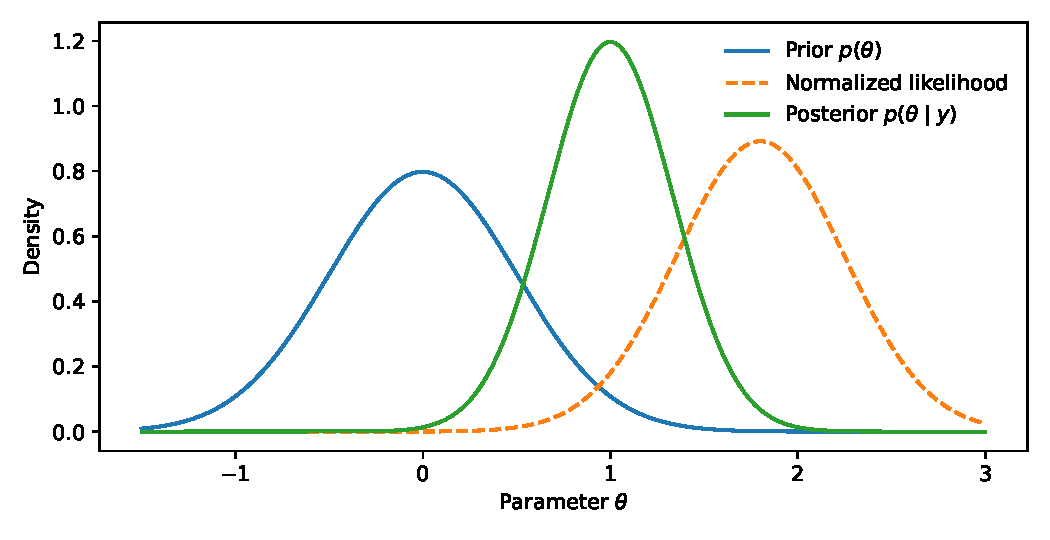
\includegraphics[width=0.82\textwidth]{fig1.pdf}
\caption{Prior density, normalized likelihood, and posterior density for the Gaussian location example.}
\label{fig:priorlikepost}
\end{figure}

\subsection{Metropolis--Hastings verification}
The unnormalized target is the product in Equation~\eqref{eq:bayestarget}. A symmetric Gaussian random walk is used in Algorithm~\ref{alg:mh}. The chain contains \(\TotalStates\) states; the first \(\BurnIn\) states are excluded, leaving \(\RetainedStates\) retained states.

\begin{figure}[ht]
\centering
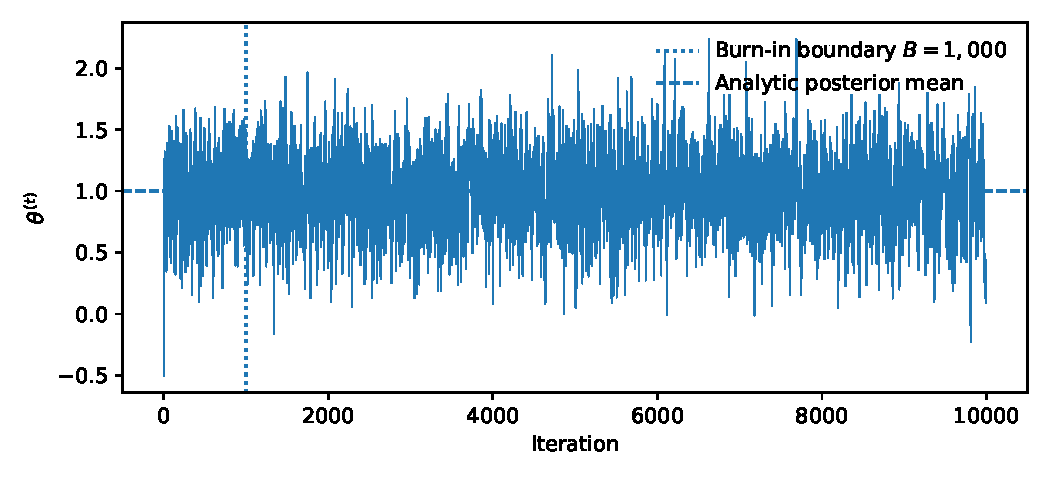
\includegraphics[width=0.82\textwidth]{fig2.pdf}
\caption{Metropolis--Hastings chain with the burn-in boundary and analytic posterior expectation.}
\label{fig:trace}
\end{figure}

The retained-state mean is \(\MHMean\), the retained-state standard deviation is \(\MHSD\), and the acceptance fraction is \(\AcceptRate\). These values are close to the analytic posterior expectation \(\PostMeanOne\) and posterior standard deviation \(\PostSDOne\).

\begin{figure}[ht]
\centering
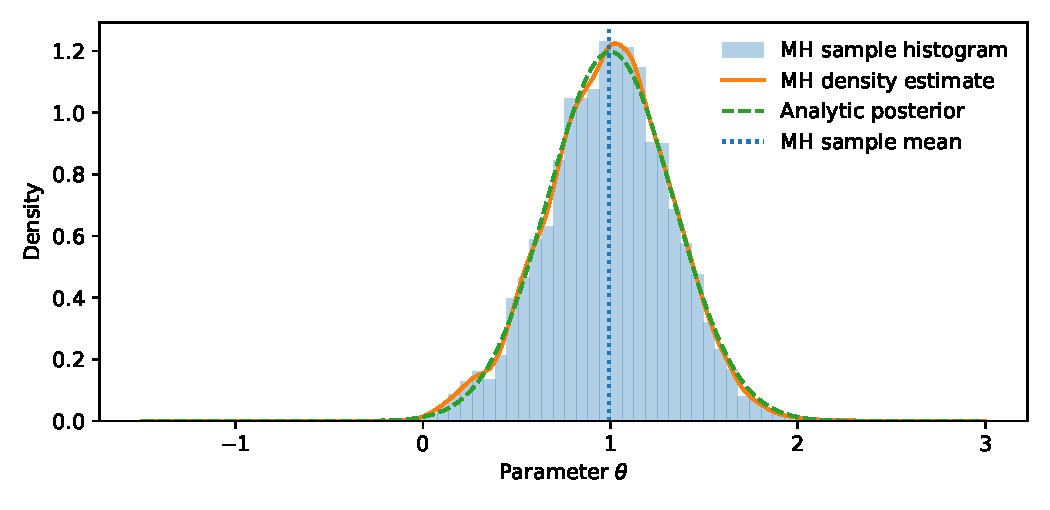
\includegraphics[width=0.82\textwidth]{fig3.pdf}
\caption{Density-normalized histogram and kernel density estimate of the retained MH states compared with the analytic posterior density.}
\label{fig:densitycomparison}
\end{figure}

\begin{figure}[ht]
\centering
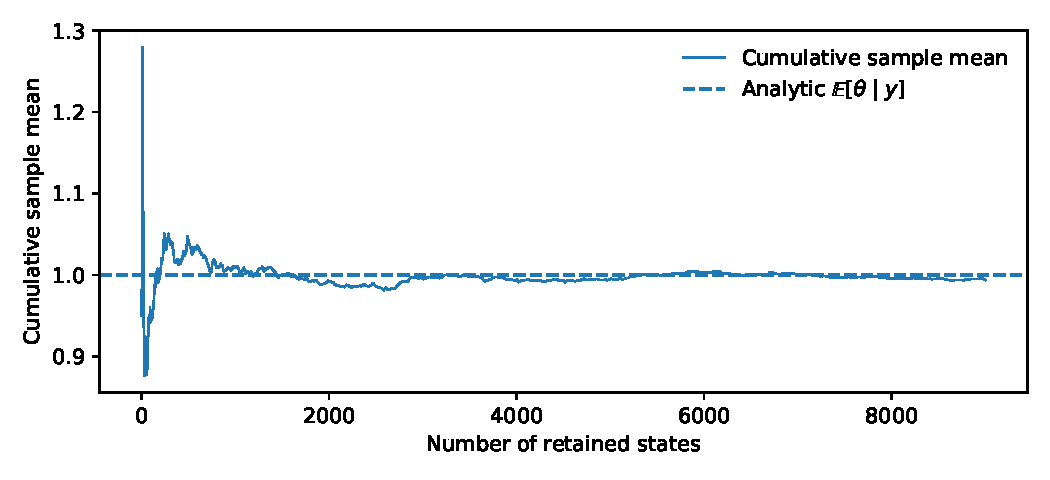
\includegraphics[width=0.82\textwidth]{fig4.pdf}
\caption{Cumulative mean of the retained states compared with the analytic posterior expectation.}
\label{fig:runningmean}
\end{figure}

\section{Example 2: scalar linear forward model}
\subsection{Model specification}
Let
\begin{equation}
 f_i(\theta)=x_i\theta,
 \qquad
 y_i=x_i\theta+\varepsilon_i,
 \qquad
 \varepsilon_i\sim\mathcal N(0,\sigma^2),
 \label{eq:linearforward}
\end{equation}
with prior
\begin{equation}
 \theta\sim\mathcal N(\mu_0,\tau_0^2).
\end{equation}
The posterior is
\begin{equation}
 \theta\mid y\sim\mathcal N(\mu_n,\tau_n^2),
\end{equation}
where
\begin{equation}
 \tau_n^2=
 \left(\frac{1}{\tau_0^2}+\frac{\sum_i x_i^2}{\sigma^2}\right)^{-1},
 \qquad
 \mu_n=\tau_n^2
 \left(\frac{\mu_0}{\tau_0^2}+\frac{\sum_i x_i y_i}{\sigma^2}\right).
 \label{eq:linearpostparams}
\end{equation}
The quantities \(\sum_i x_i^2\) and \(\sum_i x_i y_i\) enter directly into Equation~\eqref{eq:linearpostparams}. Appendix~\ref{app:linear} derives this equation from the Gaussian residual likelihood.

\subsection{Numerical evaluation}
Use \(\mu_0=0\), \(\tau_0=1\), \(\sigma=0.40\),
\begin{equation}
 x=(-2.5,-1.5,-0.5,0.5,1.5,2.5),
\end{equation}
and
\begin{equation}
 y=(-0.85,-1.05,0.05,0.55,0.45,1.75).
\end{equation}
For these observations,
\begin{equation}
 \sum_i x_i^2=\Sxx,
 \qquad
 \sum_i x_i y_i=\Sxy.
\end{equation}
Substituting these two values into Equation~\eqref{eq:linearpostparams} gives
\begin{equation}
 \theta\mid y\sim\mathcal N(\PostMeanTwo,\PostSDTwo^2).
 \label{eq:linearpostnumeric}
\end{equation}
Thus the posterior expectation of the slope is
\begin{equation}
 \mathbb E[\theta\mid y]=\PostMeanTwo.
\end{equation}

Figure~\ref{fig:linearupdate}(a) plots the prior density \(p(\theta)\) and posterior density \(p(\theta\mid y)\), together with vertical lines at the scalar expectations \(\mathbb E[\theta]\) and \(\mathbb E[\theta\mid y]\). Figure~\ref{fig:linearupdate}(b) evaluates the deterministic model \(f(x,\theta)=x\theta\) at those expectations. The shaded regions are obtained by propagating the central 95\% credible intervals for \(\theta\) through \(f\). They describe uncertainty in the deterministic model response due to uncertainty in \(\theta\); they do not include observation noise.

For fixed \(x\), if \(\theta\) has standard deviation \(s_\theta\), then \(x\theta\) has standard deviation \(|x|s_\theta\). Therefore the model-response bands collapse at \(x=0\) and widen symmetrically as \(|x|\) increases.

\begin{figure}[ht]
\centering
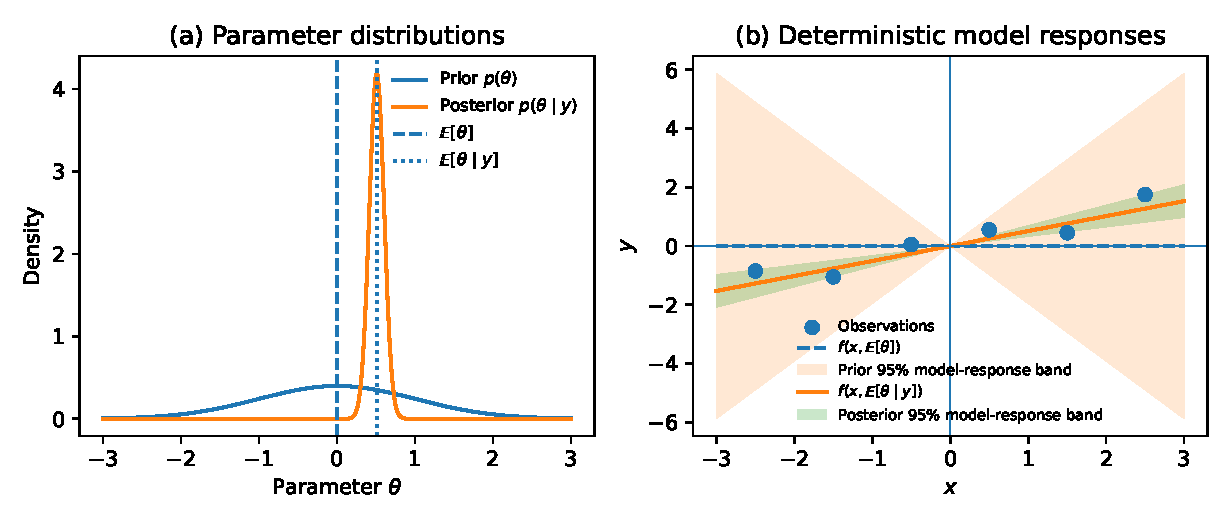
\includegraphics[width=0.98\textwidth]{fig5.pdf}
\caption{Bayesian update for the scalar linear forward model. Panel (a) shows distributions of the parameter. Panel (b) shows deterministic model responses obtained from summaries and credible intervals of those distributions.}
\label{fig:linearupdate}
\end{figure}

\section{Summary}
Bayesian inference combines a prior and a likelihood to form a posterior distribution. Metropolis--Hastings samples that posterior without requiring its normalizing constant. Its acceptance rule enforces detailed balance, which makes the posterior stationary. For deterministic forward models, a probabilistic assumption about additive errors defines the likelihood; Gaussian errors lead to a residual-sum-of-squares likelihood. The two examples permit direct comparison between analytic posterior distributions and numerical MH output.

\appendix
\part{Appendix: derivations and interpretation}

\section{How prior information and evidence are weighted}
\label{app:weighting}
For the Gaussian location model, define prior precision \(\lambda_0=1/\tau_0^2\) and likelihood precision \(\lambda_L=n/\sigma^2\). Equation~\eqref{eq:ex1postparams} can be written
\begin{equation}
 \mu_n=\frac{\lambda_0}{\lambda_0+\lambda_L}\mu_0
 +\frac{\lambda_L}{\lambda_0+\lambda_L}\bar y.
\end{equation}
The posterior expectation is therefore a weighted average of the prior expectation and the likelihood center. If \(\lambda_L\gg\lambda_0\), the posterior is close to the normalized likelihood. If \(\lambda_0\gg\lambda_L\), it remains close to the prior. Comparable precisions give substantial influence to both. The posterior precision is additive:
\begin{equation}
 \frac{1}{\tau_n^2}=\lambda_0+\lambda_L,
\end{equation}
so the posterior is narrower than either source considered separately.

\section{Completing the square for a Gaussian kernel}
\label{app:square}
A density kernel of the form
\begin{equation}
 \exp\left[-\frac12(A\theta^2-2B\theta)\right],
 \qquad A>0,
\end{equation}
can be identified as Gaussian by rewriting the quadratic expression:
\begin{align}
 A\theta^2-2B\theta
 &=A\left(\theta^2-2\frac{B}{A}\theta\right)\\
 &=A\left[\left(\theta-\frac BA\right)^2-\left(\frac BA\right)^2\right].
\end{align}
The final term is constant with respect to \(\theta\) and is absorbed into the normalization. The remaining kernel is
\begin{equation}
 \exp\left[-\frac{A}{2}\left(\theta-\frac BA\right)^2\right],
\end{equation}
which is Gaussian with mean \(B/A\) and variance \(1/A\).

\section{Gaussian location posterior derivation}
\label{app:gaussianmean}
From Equation~\eqref{eq:ex1model}, the posterior kernel is
\begin{align}
 p(\theta\mid y)
 &\propto
 \exp\left[-\frac{(\theta-\mu_0)^2}{2\tau_0^2}
 -\frac{1}{2\sigma^2}\sum_{i=1}^{n}(y_i-\theta)^2\right].
\end{align}
Expand only terms containing \(\theta\) and collect powers of \(\theta\):
\begin{equation}
 p(\theta\mid y)\propto
 \exp\left\{-\frac12\left[
 \left(\frac1{\tau_0^2}+\frac n{\sigma^2}\right)\theta^2
 -2\left(\frac{\mu_0}{\tau_0^2}+\frac{n\bar y}{\sigma^2}\right)\theta
 \right]\right\}.
\end{equation}
Applying Appendix~\ref{app:square} gives Equation~\eqref{eq:ex1postparams}.

\section{Linear forward-model posterior derivation}
\label{app:linear}
For Equation~\eqref{eq:linearforward},
\begin{equation}
 p(\theta\mid y)\propto
 \exp\left[-\frac{(\theta-\mu_0)^2}{2\tau_0^2}
 -\frac{1}{2\sigma^2}\sum_i(y_i-x_i\theta)^2\right].
\end{equation}
Expanding terms that depend on \(\theta\) gives
\begin{equation}
 \sum_i(y_i-x_i\theta)^2
 =\sum_i y_i^2-2\theta\sum_i x_i y_i+\theta^2\sum_i x_i^2.
\end{equation}
After dropping \(\sum_i y_i^2\), which is constant with respect to \(\theta\), the posterior kernel becomes
\begin{equation}
 \exp\left\{-\frac12\left[
 \left(\frac1{\tau_0^2}+\frac{\sum_i x_i^2}{\sigma^2}\right)\theta^2
 -2\left(\frac{\mu_0}{\tau_0^2}+\frac{\sum_i x_i y_i}{\sigma^2}\right)\theta
 \right]\right\}.
\end{equation}
Applying Appendix~\ref{app:square} gives Equation~\eqref{eq:linearpostparams}.

\end{document}
